
%!TEX ROOT=main.tex
\begin{figure}[ht]
\centering
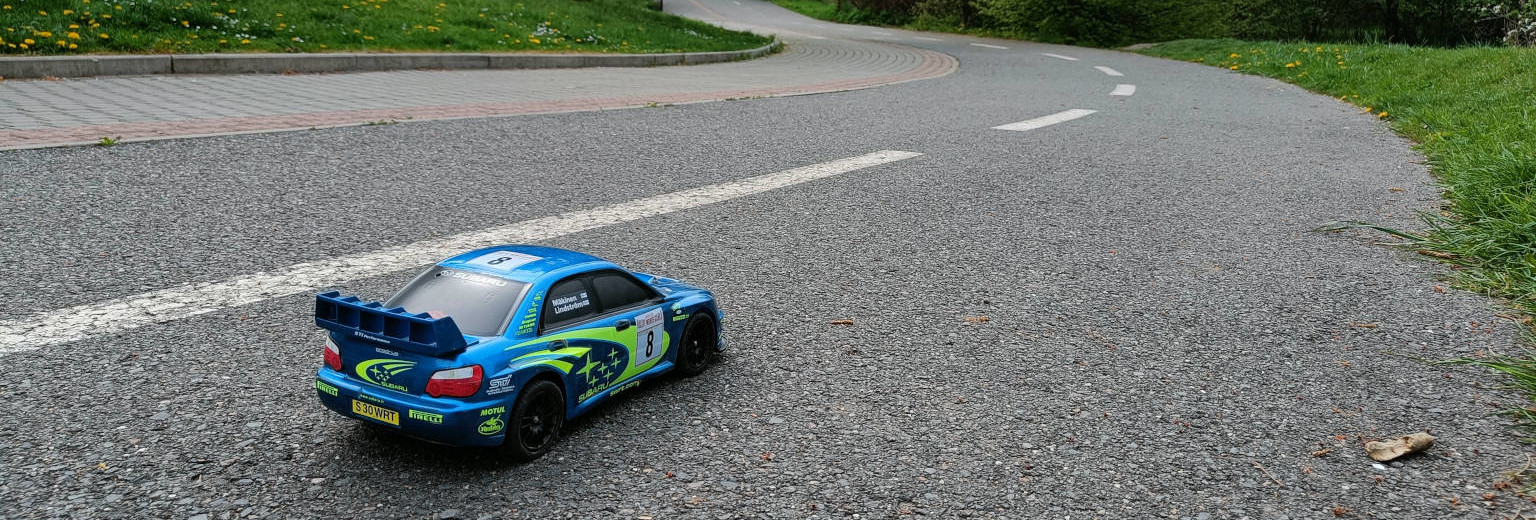
\includegraphics[width=0.8\linewidth]{fig/car.jpg}
%\caption{Used chassis}
\end{figure}
\part{Introduction}
\label{chap:intro}
\begin{myparindent}{20pt}
This thesis focuses on utilizing STM32 microcontrollers to design and build an RC car control board. As the project is Radio Controlled, a control device - a transmitter - had to be developed as well. Both devices are constructed primarily from available modules, which were sometimes modified and combined to form a working RC system.
\end{myparindent}

Therefore, the thesis contains the development of both devices and describes the functional blocks used. The necessary control software, which was developed for both devices, is also presented and explained in detail. Finally, the designed system was tested in real conditions.

The proposed car control system is retrofitted to a particular chassis, but the application of a standard RC control signal using PWM makes it possible to mount the control board to a different chassis with a different servo and motor.

\section{Motivation}
The main motivation was to build an RC car with an STM32 microcontroller that would function and behave like a regular RC car, but at the same time, would be extraordinary. Extraordinary, for example, in terms of range, non-standard features, or user customizability.

Most commercially available RC systems are proprietary and closed and use undocumented components, thus making the modification hard or even impossible. Some hardware modifications are possible with expensive accessories, but the control software customization is usually impossible even with the accessories. This prohibits, for example, advanced driving data reporting and recording or the use of custom sensors.

The solution proposed in this thesis solves the problem, as control boards are built from available and community-known modules, and the control software written in C language is open-source. Additionally, the car control board contains various sensors and a micro SD card slot to record driving data, which can be later visualized and analyzed.

Since the project is not built from scratch and as a base uses an old chassis and transmitter with no spare parts available, another motivation was to make all the modifications with minimal physical intervention to reduce the risk of irreversibly breaking it.



